\section{Analiza opóźnień wprowadzanych przez metody obrony}
W następnym etapie przeanalizowano narzut obliczeniowy wprowadzany przez badane metody mitygacji podatności w stosunku do poziomu bazowego. Latencję badano przy użyciu metryk \gls{TTFT} oraz \gls{TBT}. W eksperymencie wykorzystano losowy podzbiór 50 bezpiecznych zapytań z JBB-Behaviours~\cite{chao2024jailbreakbenchopenrobustnessbenchmark}. Sprawdzenie opóźnień na zapytaniach szkodliwych skutkowałoby przedwczesnym przerwaniem generacji odpowiedzi, co uniemożliwiłoby realne porównanie czasu generacji tokenów dla dłuższych odpowiedzi. Odmowy nie były wliczane do metryk strumieniowania. Długość generowanych odpowiedzi przez model ograniczono do 128 tokenów. By móc porównać ze sobą wszystkie metody na podstawie metryk \gls{TTFT} i \gls{TBT}, użyto wariantu obrony przy użyciu Llama-Guard sprawdzającego jedynie wejście, zamiast dodatkowo odpowiedź modelu docelowego. Drugi wariant nie pozwolił na porównanie statystyk strumieniowania, gdyż generacja odpowiedzi nie jest zwracana użytkownikowi do momentu jej ukończenia i finalnej weryfikacji przez model moderujący. W celu zminimalizowania wpływu środowiska na pomiary, przed pętlą pomiarową dla każdej metody obrony zadano inicjalizujące polecenie, które miało na celu wyeliminowanie jednorazowych opóźnień, przykładowo alokacja przestrzeni VRAM. Ponadto, każdy prompt ewaluowano trzykrotnie. Dodatkowo, kolejność wywoływania metod obrony była w każdej iteracji losowa. Do analizy opóźnień wykorzystano także miary takie jak mediana (p50), która reprezentowała standardową responsywność systemu oraz percentyle p90 i p99, które służyły do wykrywania anomalii czasowych.
\begin{table}[htbp]
    \centering
    \renewcommand{\arraystretch}{1.2}
    \begin{tabular}{l|c|c|c|c|c|c}
        \hline
        \multirow{2}{*}{\textbf{Metoda obrony}} & \multicolumn{3}{c|}{\textbf{TTFT [ms]}} & \multicolumn{3}{c}{\textbf{TBT [ms]}}                                                             \\\cline{2-7}
                                                & \textbf{p50}                            & \textbf{p90}                          & \textbf{p99} & \textbf{p50} & \textbf{p90} & \textbf{p99} \\\hline
        Poziom bazowy                           & 40,7                                    & 43,3                                  & 46,4         & 33,3         & 33,6         & 36,3         \\\hline
        Self-Reminder                           & 41,4                                    & 44,0                                  & 50,8         & 33,4         & 33,7         & 36,6         \\\hline
        Llama-Guard (na wejściu)                & 428,4                                   & 443,3                                 & 471,9        & 33,3         & 33,7         & 36,2         \\\hline
        Sterowanie aktywacjami                  & 41,6                                    & 46,2                                  & 52,0         & 33,3         & 33,6         & 36,2         \\\hline
    \end{tabular}
    \caption{Zestawienie statystyk opóźnień TTFT oraz TBT dla badanych metod mitygacji dla modelu Llama-3.1-8B-Instruct}
    \label{tab:latency_metrics_llama}
\end{table}

\begin{table}[htbp]
    \centering
    \renewcommand{\arraystretch}{1.2}
    \begin{tabular}{l|c|c|c|c|c|c}
        \hline
        \multirow{2}{*}{\textbf{Metoda obrony}} & \multicolumn{3}{c|}{\textbf{TTFT [ms]}} & \multicolumn{3}{c}{\textbf{TBT [ms]}}                                                             \\\cline{2-7}
                                                & \textbf{p50}                            & \textbf{p90}                          & \textbf{p99} & \textbf{p50} & \textbf{p90} & \textbf{p99} \\\hline
        Poziom bazowy                           & 38,8                                    & 43,6                                  & 46,6         & 36,4         & 37,5         & 40,0         \\\hline
        Self-Reminder                           & 42,9                                    & 46,3                                  & 51,8         & 36,5         & 37,6         & 40,5         \\\hline
        Llama-Guard (na wejściu)                & 428,5                                   & 439,4                                 & 507,7        & 36,3         & 37,3         & 40,0         \\\hline
        Sterowanie aktywacjami                  & 40,0                                    & 43,8                                  & 48,3         & 36,5         & 37,9         & 40,6         \\\hline
    \end{tabular}
    \caption{Zestawienie statystyk opóźnień TTFT oraz TBT dla badanych metod mitygacji dla modelu Mistral-7B-Instruct-v0.3}
    \label{tab:latency_metrics_mistral}
\end{table}
Na podstawie danych zawartych w tabelach~\ref{tab:latency_metrics_llama} oraz~\ref{tab:latency_metrics_mistral} można zauważyć, że metoda obrony oparta na sterowaniu aktywacjami zwiększa medianę opóźnienia \gls{TTFT} o zaledwie 0,9 ms dla modelu Llama oraz 1,2 ms dla modelu Mistral. Wskazuje to na nikły narzut metody na czas zainicjowania generacji odpowiedzi, a z perspektywy doświadczenia użytkownika końcowego jest to zmiana niedostrzegalna. Analizując wartości p90 oraz p99 metryki \gls{TTFT} dla sterowania aktywacjami można dojść do wniosku, że nawet z najgorszych zarejestrowanych przypadkach pod względem czasowym, narzut obliczeniowy jest wciąż mało istotny w porównaniu do poziomu bazowego. Różnica tej metryki między p99 w scenariuszu bez metody obrony a p99 dla sterowania aktywacjami wynosi 1,7 ms dla modelu Mistral, natomiast dla modelu Llama 5,6 ms. Technika ta wykazała również stabilne rezultaty czasu między kolejnymi tokenami otrzymując rezultat niemal identyczny jak dla poziomu bazowego.

Jeśli chodzi o metodę obrony Self-Reminder, wprowadziła ona akceptowalne opóźnienie w generacji pierwszego tokena, które wyniosło 0,7 ms dla modelu Llama oraz nieco większe opóźnienie w modelu Mistral wynoszące 4,1 ms. Narzut ten może być spowodowany przetwarzaniem instrukcji systemowej i sufiksu, które zwiększają wypełnienie okna kontekstowego. Dla tej metody opóźnienia p99 dla \gls{TTFT} wzrosły z 46,4 ms do 50,8 ms dla modelu Llama i z 46,6 ms do 51,8 ms dla modelu Mistral. Natomiast dla p90 różnice te wyniosły odpowiednio 1,3 ms i 2,7 ms. Metoda ta również uzyskała wyniki \gls{TBT} bardzo zbliżone do poziomu bazowego.

Natomiast wykorzystanie na wejściu modelu moderującego Llama-Guard spowodowało zauważalny narzut, który można dostrzec podczas analizy wyników \gls{TTFT}. Dla obu modeli mediana tej miary wzrosła do około 428,5 ms, co stanowi wzrost dziesięciokrotny w stosunku do scenariusza bez tej metody mitygacji. Uwarunkowane jest to koniecznością przetworzenia promptu wejściowego przez Llama-Guard przed zainicjowaniem generacji przez model docelowy. W 1\% najgorszych rezultatów dla modelu Llama opóźnienie to było na poziomie 471,9 ms, co stanowi wzrost o ponad 40 ms od mediany. Natomiast dla modelu Mistral wartość ta była równa 507,7 ms, co stanowi najgorszy otrzymany wynik p99 \gls{TTFT} w niniejszych badaniach. Oznacza to że użytkownik końcowy przeciętnie dostrzegałby opóźnienie na poziomie 0,43 s, a w najgorszych przypadkach ponad pół sekundy. Natomiast metoda ta osiąga zadowalające wartości metryki \gls{TBT}, które są porównywalne do poziomu bazowego. Dostrzec można, że każda z metod nie wprowadza narzutu na czas między kolejnymi wygenerowanymi tokenami.

Pełniejszy obraz charakterystyki czasowej zapewniają dystrybuanty empiryczne przedstawione na wykresach~\ref{fig:ecdf_comparison_llama} i~\ref{fig:ecdf_comparison_mistral}.

\begin{figure}[htbp]
    \centering
    \begin{subfigure}[b]{0.48\textwidth}
        \centering
        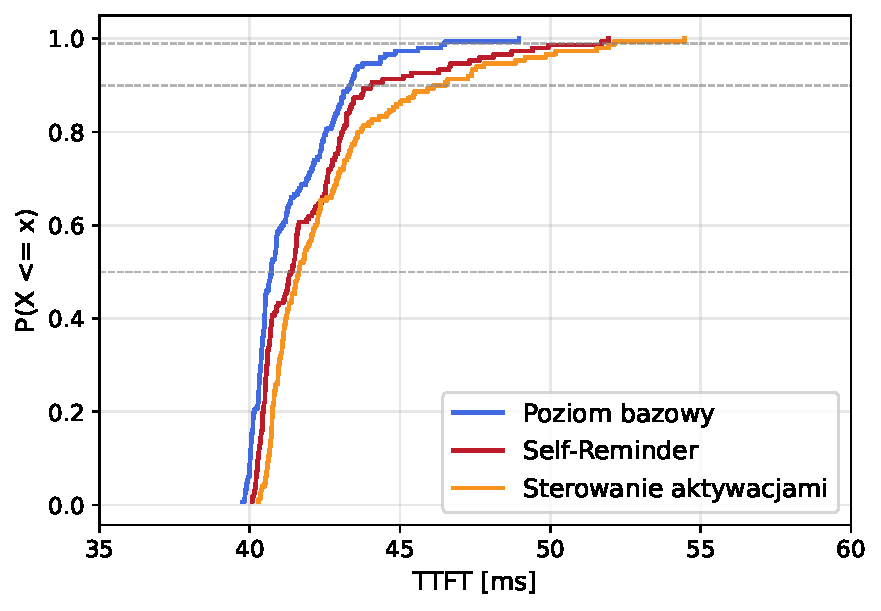
\includegraphics[width=\linewidth]{diagramy/ecdf_others_ttft_llama.pdf}
        \label{fig:ecdf_others_llama}
    \end{subfigure}
    \hfill
    \begin{subfigure}[b]{0.48\textwidth}
        \centering
        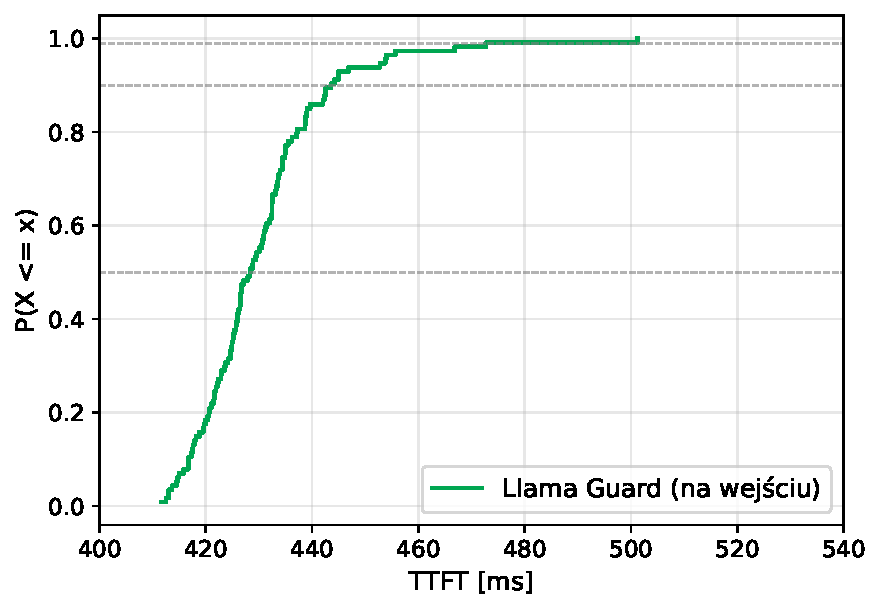
\includegraphics[width=\linewidth]{diagramy/ecdf_guard_ttft_llama.pdf}
        \label{fig:ecdf_guard_llama}
    \end{subfigure}
    \caption{Porównanie dystrybuant empirycznych dla metryki TTFT dla metod obrony modelu Llama-3.1-8B-Instruct}
    \label{fig:ecdf_comparison_llama}
\end{figure}

\begin{figure}[htbp]
    \centering
    \begin{subfigure}[b]{0.48\textwidth}
        \centering
        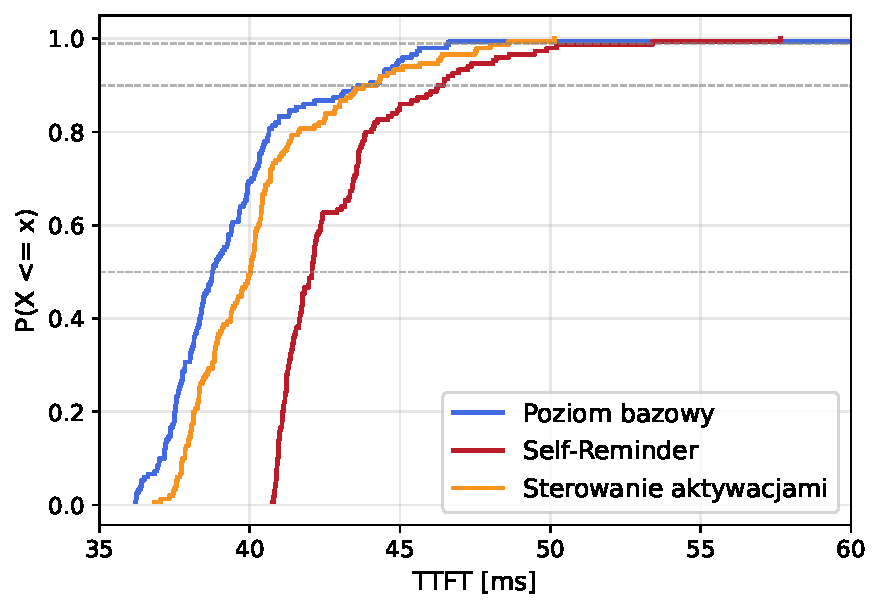
\includegraphics[width=\linewidth]{diagramy/ecdf_others_ttft.pdf}
        \label{fig:ecdf_others_mistral}
    \end{subfigure}
    \hfill
    \begin{subfigure}[b]{0.48\textwidth}
        \centering
        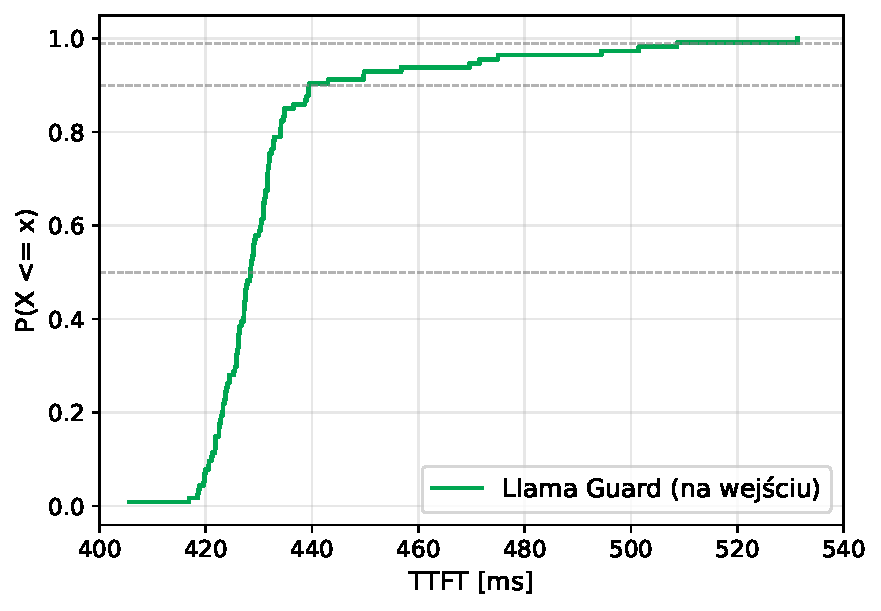
\includegraphics[width=\linewidth]{diagramy/ecdf_guard_ttft.pdf}
        \label{fig:ecdf_guard_mistral}
    \end{subfigure}
    \caption{Porównanie dystrybuant empirycznych dla metryki TTFT dla metod obrony modelu Mistral-7B-Instruct-v0.3}
    \label{fig:ecdf_comparison_mistral}
\end{figure}

Zweryfikowano również czas pełnej odpowiedzi dla metody obrony przy pomocy weryfikacji intencji przez Llama-Guard zarówno na wejściu jak i wyjściu. Metryki \gls{TBT} oraz \gls{TTFT} zastąpiono w tym przypadku \gls{TTFR}, czyli miarą czasu pełnej odpowiedzi systemu. Mediana tego czasu wyniosła 4993,9 ms, czyli w przybliżeniu 5 s. Natomiast percentyl p90 wyniósł 5039,5 ms, a p99 był równy 5112,9 ms. Ponadto, analiza zapytań odrzuconych na wejściu wykazała, że mediana czasu odmowy wykonania polecenia wyniosła 694,6 ms, a w 1\% najgorszych przypadków 775,5 ms. Dostrzegalną różnicą przy wdrożeniu tej metody jest doświadczenie użytkownika końcowego, ponieważ oczekuje on około 5 s na otrzymanie w pełni wygenerowanej odpowiedzi. Natomiast w przypadku innych badanych metod obrony, takich jak Self-Reminder oraz techniki sterowania aktywacjami, użytkownik otrzymuje pierwszy token po około 41 ms i przez pozostały czas może na bieżąco analizować generowaną odpowiedź.